\begin{figure}[!ht]
 \begin{center}
  \subfigure[]{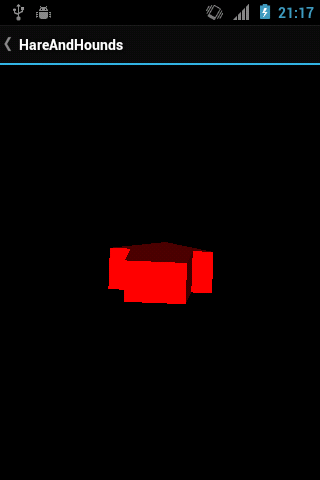
\includegraphics[width=0.2\textwidth]{figures/spaceGraphics_orientation_VerN.png}}
  \subfigure[]{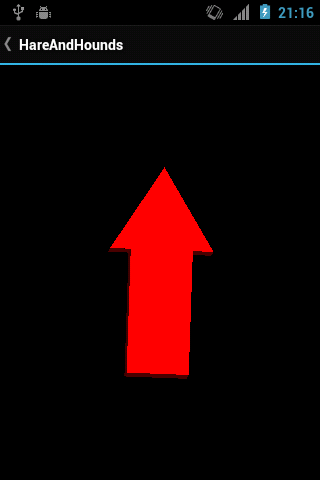
\includegraphics[width=0.2\textwidth]{figures/spaceGraphics_orientation_HorN.png}}\\
  \subfigure[]{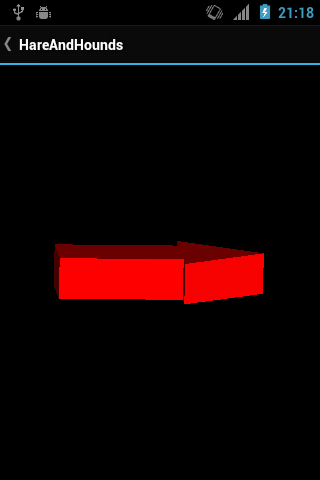
\includegraphics[width=0.2\textwidth]{figures/spaceGraphics_orientation_VerW.png}}
  \subfigure[]{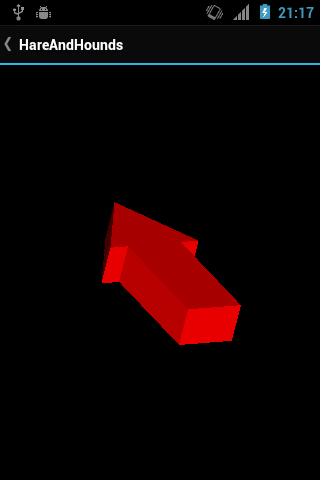
\includegraphics[width=0.2\textwidth]{figures/spaceGraphics_orientation_mixed.png}}
 \end{center}
 \caption{
  Przykłady obróconego modelu strzałki wsazującej północ:
  (a) telefon trzymany pionowo, skierowany na północ;
  (b) telefon leżący poziomo, skierowany na północ;
  (c) telefon trzymany pionowo, skierowany na zachód;
  (d) telefon skierowany lekko w dół i~na prawo od północy.
 }
 \label{fig:spaceGraphics_orientation}
\end{figure}
